\documentclass[conference]{IEEEtran}
\usepackage[table]{xcolor}
\usepackage[english]{babel}
\usepackage[utf8]{inputenc}
\usepackage[style=numeric]{biblatex}
\usepackage{amsmath}
\addbibresource{../literature.bib}% Syntax for version >= 1.2
\usepackage{graphicx}
\graphicspath{{../images/}}
\usepackage{multirow}

% circles
\usepackage{wasysym}
\newcommand{\Tdot}{$\CIRCLE$}
\newcommand{\Thdot}{$\LEFTcircle$}
\newcommand{\Twdot}{$\Circle$}

% for fancy table with rotated column titles
\usepackage{tabularx}
\usepackage{adjustbox}
\newcolumntype{R}[2]{%
    >{\adjustbox{angle=#1,lap=\width-(#2)}\bgroup}%
    l%
    <{\egroup}%
}
\newcommand*\rot{\multicolumn{1}{R{45}{0.01em}}}% no optional argument here, please!
\newcommand*\rota{\multicolumn{1}{R{90}{0.01em}}}% no optional argument here, please!
\def\hb{\hbox to 10.7 cm{}}

%colors in tables
\definecolor{abfred}{RGB}{255, 215, 215}
\definecolor{abf-rg-1}{RGB}{251,213,242}
\definecolor{abf-rg-2}{RGB}{243,212,249}
\definecolor{abf-rg-3}{RGB}{213,210,245}
\definecolor{abf-rg-4}{RGB}{208,231,242}
\definecolor{abf-rg-5}{RGB}{206,238,223}
\definecolor{abf-rg-6}{RGB}{205,236,210}
\definecolor{abf-rg-7}{RGB}{211,234,204}
\definecolor{abfgreen}{RGB}{221,232,203}
\definecolor{abforange}{RGB}{255, 245, 206}

%fix commands
\newcommand{\fixnote}[2]{\textbf{\color{red}{FIX}}\footnote{{\bf #1:} #2}}
\newcommand{\fix}[2]{{\color{red} {\bf tofix:} #2}}
% \renewcommand{\fixnote}[2]{}
% \renewcommand{\fix}[2]{}

\newcommand{\assertionRegion}{\mathcal{A}}
\newcommand{\beliefRegion}{\mathcal{B}}
\newcommand{\factRegion}{\mathcal{F}}
\newcommand{\rcc}{rcc}
\newcommand{\agentuniverse}{Ag}
\newcommand{\abf}{\assertionRegion,\beliefRegion,\factRegion}
\newcommand{\Rcc}[2]{rcc(#1,#2)}
\newcommand{\connects}[2]{C(#1,#2)}
\newcommand{\disconnected}[2]{\neg C(#1,#2)}
\newcommand{\partof}[2]{P(#1,#2)}
\newcommand{\overlaps}[2]{O(#1,#2)}
\newcommand{\eq}[2]{EQ(#1,#2)}
\newcommand{\pp}[2]{PP(#1,#2)}
\newcommand{\po}[2]{PO(#1,#2)}
\newcommand{\ppi}[2]{PPi(#1,#2)}
\newcommand{\dr}[2]{DR(#1,#2)}
\newcommand{\all}[2]{T(#1,#2)}
\newcommand{\rassert}[3]{\mathcal{A}_{#1\rightarrow #2}#3}
\newcommand{\lassert}[3]{\mathcal{A}_{#1\leftarrow #2}#3}

\newtheorem{definition}{Definition}%[section]

\begin{document}
\title{On Etiology of Cybersecurity}

\author{\IEEEauthorblockN{Marco Rocchetto}
\IEEEauthorblockA{V-Research\\
Verona, Italy\\
Email: marco@v-research.it}
\and
\IEEEauthorblockN{Francesco Beltramini}
\IEEEauthorblockA{V-Research\\
Verona, Italy\\
Email: francesco@v-research.it}
}

\maketitle

\begin{abstract}
The abstract goes here.
\end{abstract}

\IEEEpeerreviewmaketitle

\section{Introduction}\label{sec:intro}
In \cite{Herley2016unfalsifiability}, Cormac Herley explores what he calls
``an asymmetry in computer security'', which he defines as follows: ``Things
can be declared insecure by observation, but not the reverse. There is no
observation that allows us to declare an arbitrary system or technique
secure''. Herley then uses this argument to show that ``claims that any measure
is necessary for security are empirically unfalsifiable''. Given that, any
theory which is not falsifiable by an empirical experiment is well
known\footnote{``A theory which is not refutable by any conceivable event is
nonscientific. Irrefutability is not a virtue of a theory (as people often
think) but a vice.'' -- Karl Popper, Conjectures and
Refutations \cite{popper1962conjectures}} to be nonscientific (i.e.
unfalsifiability is a fallacy of a theory), Herley concludes that there is no
scientific theory on cybersecurity; which means that cybersecurity lays in the
realm of pseudo-sciences \cite{Herley2016usenixvideo}.  Herley, e.g.
in \cite{Herley2017justifying}, discusses the implications of a
nonscientific approach to cybersecurity, and highlights the tremendous impact on
all the scientific research and engineering of systems; leading often to
terrorism and wars, and wasting of resources in useless protections or
overspending.  While the criticism is investigated
in \cite{Herley2016unfalsifiability}, no solution is provided nor envisioned.  On the
contrary, the goal of this work is to lay the foundations of a
scientific cybersecurity theory. 

We consider the problem raised by Herley not confined to
``computer security'' but to any abstract system (so that our theory may hold
for any sound implementation such as networks, mechanical, cyber, or
cyber-physical system, or even a single computer or a single device such as an
hard-drive).  There is also an apparent inconsistency in
\cite{Herley2016unfalsifiability} that we seek to clarify before following (as
we agree) the scientific path draw by Herley: cybersecurity is defined as an
abstract property in many formal approaches to the investigation of the
security of systems, and the security of the design of a formally verified
protocol is indeed falsifiable (against the security properties verified).  For
example, in the protocol verification community, security is often defined as a
formalization of the high-level properties confidentiality, integrity, and
availability. The problem in such approaches is not the definition of what
cybersecurity is but the generality of the results, since they tackle a specific
step (and not the first) of the engineering process (of systems).  Therefore,
the theories underlying the verification are based on assumptions which
non-evidently apply to a general security theory.  As an example, the so called
Dolev-Yao attacker model\footnote{For the sake of simplicity, the Dolev-Yao
attacker can be considered as an abstraction of an active attacker who controls
the network but cannot break cryptography.} \cite{Dolev1983security} only
applies to specific instances (often called scenarios) and abstraction of the
protocol. This, in turn, creates a false sense of security since requires
non-justifiable assumptions on the abstraction of the system of which security
is verified. More specifically, for the formal security verification of a
system in which two or more agents are communicating, a formalized scenario
needs to be defined by a modeler who chooses (among others): (i) a scope of the
formalization (e.g.  excluding the server that distributes the public key is
often done when verifying the security of authentication protocols), (ii) the
number of sessions (even tough some approaches do reason on an infinite number
of sessions such as \cite{Escobar2007maudenpa}), (iii) honesty/dishonesty of
the peers (e.g.  in the ASLan++ language \cite{Oheimb2010aslan++}), and (iv)
the abstraction of the cryptographic primitives (e.g.  ProVerif vs CryptoVerif
\cite{Blanchet2017symbolic}).  While many tools and theories improves those 
issues, there is no agreement on which should be the definitive
approach (if any). More importantly, some of the choices made by the
modelers/engineers using those formal approaches may completely change the
results of the formal verification of the system (an interesting example on how
difficult it is to even just compare the approaches is given in
\cite{Cremers2009comparing}). 
\begin{figure}[t]
	\centering
	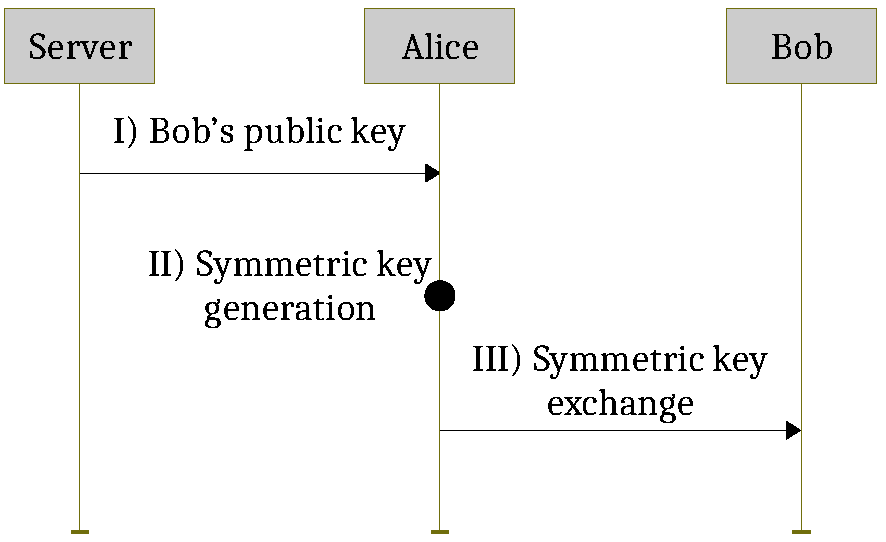
\includegraphics[width=.7\columnwidth]{protocol-example.pdf}
	\caption{Abstraction of an ad-hoc esemplificative protocol execution}
	\label{fig:protocol-example}
\end{figure}
For example, in Figure~\ref{fig:protocol-example}, under the perfect
cryptography assumption\footnote{As defined in \cite{Rocchetto2016cpdy}: ``In
the so called perfect cryptography assumption, the security encryption scheme
is suppose to be perfect, without any exploitable flaw, and so the only way for
the attacker to decrypt a message is by using the proper key. That assumption
is widely accepted in the security protocol community, and most of the formal
reasoning tools for the analysis of security protocols abstract away the
mathematical and implementation details of the encryption scheme
\cite{Turuani2006clatse,Basin2005ofmc,Armando2016satmc,Rocchetto2017interpolation}''}
and assuming that no violation to any security property is done after message
I), the freedom of choosing the scope
determines that the flaws related to the dishonest impersonation of the Server
may or may not be considered in the verification process.  This choice has
tremendous impact on the focus and findings of the verification of the security
of the protocol.  While this may seem to turn upon minutiae and foreseeable,
this highlights the false sense of security that may derive from a
non-falsifiable theory of system security\footnote{``To the superficial
observer, the analysis of these forms seems to turn upon minutiae. It does in
fact deal with minutiae, but they are of the same order as those dealt with in
microscopic anatomy.'' -- Karl Marx, Capital Volume 1, 1867}.

\paragraph{Structure} We start, in
Section~\ref{sec:literature}, by detailing the problem statement, reporting a
literature review on the main concepts and definitions related to security.  We
formulate a security hypothesis in Section~\ref{sec:hypothesis}; which we use
to propose a theory on system security in Section~\ref{sec:theory}. In
Section~\ref{sec:secra}, we apply our theory for the tool-assisted security
risk assessment of a CPS (with an ad-hoc example, based on the SWaT testbed
\cite{Mathur2016swat}).  This application shows how our theory can be used to
predict all of the possible security weaknesses of a system, allowing the
falsification of our theory.  In fact, if any security weaknesses were to be
found in a system and not predicted by our theory, the theory could be declared
incomplete.  Similarly, if a security weakness would be predicted by our theory
but found to be impossible to have our theory could be declared as wrong.

\section{Literature Review}\label{sec:literature}
\begin{figure*}[t]
	\centering
	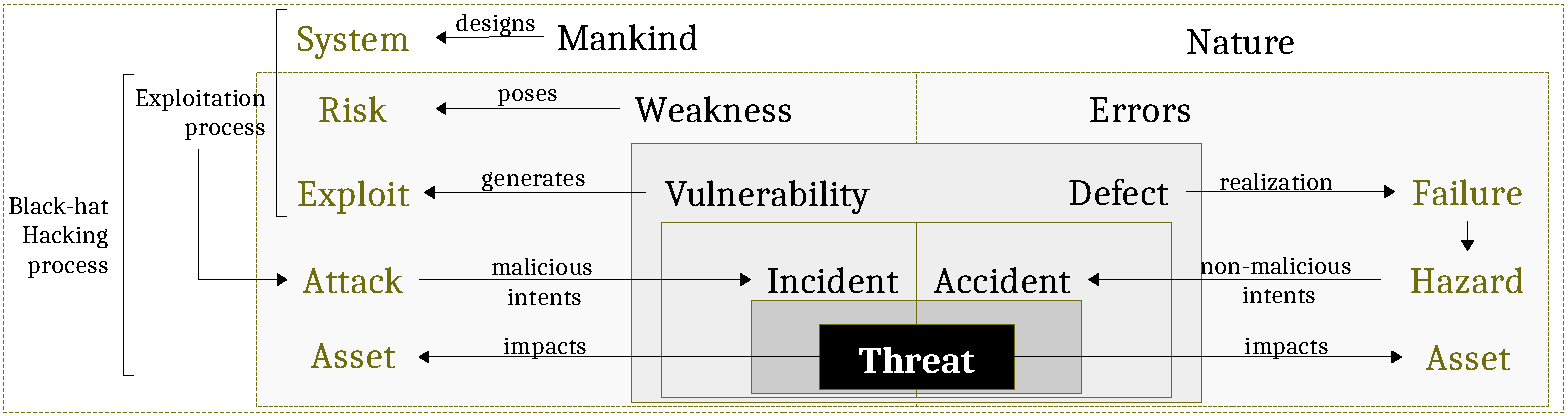
\includegraphics[width=.9\textwidth]{safety-security_3.pdf}
	\caption{Overview of keywords related to security and safety}
	\label{fig:safety-security}
\end{figure*}

\fixnote{mr}{add weakness-error in picture and text}
In most of the natural languages the concepts of safety
and security are not syntactically differentiated and both terms (safety and
security) are expressed by the same word, e.g. sicurezza in Italian.  A
semantic distinction between safety and security is correlated to a
belief\footnote{A belief has to be intended as a proposition which is supposed
to be true by the majority of people in our society, without a scientific
underlying theory but based on partial empirical evidences or inductive reasoning based on partial empirical evidences.} that
safety deals with \emph{accidents} (i.e. an unfortunate incident) posed by the
natural environment (e.g. natural events such as wearing of hardware
components) while security deals with \emph{incidents} posed by mankind (e.g.
attackers and bugs).  The fundamental difference between nature and mankind (and,
in turn, between safety and cybersecurity) is believed to be on the different
intents\footnote{``The belief–desire–intention software model (BDI) is a
software model developed for programming intelligent
agents.''\cite{wiki-bdi}. In the BDI model, the intents represents the
deliberative state of an agent which determines the choice of that agent on
what to do.} (accidents are unfortunate while incidents are not) of the causes
that generates a threat; namely, nature is believed not to have malicious
intents (but unfortunate causes-effects) while threats generated by mankind are
malicious\footnote{Of course, logical flaws or bugs may be
introduced by other means (e.g. ignorance) without explicit malicious intents,
but the exploitation of those flaws is considered (for now, and detailed
afterwards in the article) malicious, and then we consider any vulnerability to
be malicious even if due to the lack of skills.}.
This conclusion seems to be against a general formulation of a cybersecurity theory;
how can we define a theory that predicts what a human being will do?
The cybersecurity attacks seems to be related to the creativity of the attacker
and then unpredictable. Currently, our understanding of cybersecurity is
stored into a network of databases of weaknesses (e.g.
CWE\cite{MITRE2020CWEresearch}), vulnerabilities (e.g. CVE\cite{CVE},
NVD\cite{NIST2020NVD}),
and attacks (e.g. CAPEC\cite{MITRE2020CAPEC}, ATTACK\cite{attack}). Systems are
nowadays tested against 
known attacks ignoring the fact that the considering a system secure
if no known attack is possible, defines an unfalsifiable claim.
As an example, if we have a system which is secure against all of the
vulnerabilities in the CVE we just need to wait for a month to have 1000+ more
vulnerabilities to test \cite{newVulns}. If we suppose that one of those new vulnerabilities
affects our system, that should be the falsification of the hypothesis that a
system is secure if no known attacks apply. So, even tough the field 
of security protocols is still lacking of a general cybersecurity theory
the secure-by-design approach they apply can be considered as going
into the opposite direction of the ``implement and test'' approach.

Most of the safety-preserving principles in the field of engineering of
safety-critical cyber-physical systems (such as elevators and aircraft), upon
which safety requirements are defined (e.g. in standards such as the IEC 61508
or 61511\cite{IEC201761511}), are based on empirical tests and measurements
(therefore should be considered hypothesis and not definitions). While
reasoning by induction\footnote{``So, whenever they argue ``Every man is an
animal and Socrates is a man; therefore Socrates is an animal,'' proposing to
deduce from the universal proposition ``every man is an animal'' the particular
proposition ``Socrates therefore is an animal,'' which in fact goes (as we have
mentioned) to establish by way of induction the universal proposition, the
fall into the error of circular reasoning, since they are establishing the
universal proposition inductively by means of each of the particulars and
deducing the particular proposition from the universal syllogistically.''
Sextus Empiricus, Outlines of Pyrrhonism II-195 \cite{Empiricus1990Pyrrhonism}}
based on the empirical observation should be avoided, since it may easily lead
to false beliefs, this approach is often justified by the supposed
impossibility of defining a theory that correctly predicts failures.  A failure
of a wire due to environment (e.g. due to humidity, dust, heat \&c) is defined
from empirical evidences and processes have been standardized to test qualities
of hardware components.  This process completely breaks down when a malicious
environment (i.e. an attacker) is considered instead of the (supposedly honest
and predictable) natural environment. Therefore, the same approach that is in
use for safety, seems not to be applicable for security (e.g. for security
testing).
An overview on the aforementioned aspects of safety and security is depicted in
Figure~\ref{fig:safety-security} and is used as a baseline for a definition of
the terms that structure our current understanding of security. 
\begin{itemize}
	\item \emph{Mankind} ``refers collectively to humans''
\cite{wiki-mankind}, while the concept of \emph{Nature} is
		related ``to the intrinsic characteristics that plants,
		animals, and other features of the world develop of their own
		accord'' (e.g. the physical universe)\cite{wiki-nature}. 
		\begin{itemize}
			\item There exist several terms to refer to an
				\emph{attacker}, i.e. threat agent or threat source,
				considering those terms to be semantically
				equivalent.  From now on, we consider the
				Causality principle to be the \emph{threat
				source}, Nature or Mankind to be the
				\emph{threat agents} and an \emph{attacker} as
				a specific malicious threat agent which materializes a
				threat.
		\end{itemize}
	\item \emph{Vulnerability}\footnote{The term vulnerability is not
		present in the Encyclopedia of Cryptography and Security, while
		it is used in 12 entries (such as in the definition of
		``penetration testing'' \cite{caddy2005pentest})
		highlighting how commonly this word is used without a proper
		supporting semantics.}, as defined in \cite{cnssi20104009}
		(and adopted in \cite{nist2013800-53}), is ``weakness in an
		information system, system security procedures, internal
		controls, or implementation that could be exploited by a threat
		source''. On the one hand, the definition is broad to enclose
		as much causes (that generates a vulnerability) as possible
		On the other hand, the term vulnerability should have a complete and sound
		definition, so that no other causes (e.g.  other sources) but
		the ones in the definition are responsible for a vulnerability
		\footnote{``For this view, that
		\emph{That Which Is Not} exists, can never predominate. You
		must debar your thought from this way of search, nor let
		ordinary experience in its variety force you along this way,
		(namely, that of allowing) the eye, sightless as it is, and the
		ear, full of sound, and the tongue, to rule; but (you must)
		judge by means of the Reason (Logos) the much-contested proof
		which is expounded by me.'' -- Parmenides of Elea, On Nature
		(circa 500 B.C.), fragments B7.1–8.2
		\cite{Hakim2016philosophy}}.
		Furthermore, the term ``threat sources'' used in the definition
		in\cite{cnssi20104009} may be identified with both Nature
		and Mankind, not differentiating between safety and security.
\end{itemize}

As depicted in Figure~\ref{fig:safety-security}, a vulnerability does not
necessarily become a threat for the system, unless exploited ``through a
channel that allows the violation of the security policy
[\ldots]''\cite{cnssi20104009}. For example, a software or procedure that takes
advantage of the vulnerability causing an \emph{attack} to the system may
result in several correlated incidents and threats.  The process of
exploitation of a defect as a vulnerability is reported in
Figure~\ref{fig:safety-security} such that the difference between exploit and failure,
and attack and accident, is to be found just in the maliciousness of the intents
that causes this process (i.e. excluding the intent, the terms are just syntactic transformation from a vulnerability to defect, from
accident to incident). 

\begin{itemize}
	\item \emph{Weakness}. The definition given by the MITRE
		in \cite{MITRE2020CWEweakness} of weakness is: ``Software
		weaknesses are errors that can lead to software
		vulnerabilities. A software vulnerability, such as those
		enumerated on the Common Vulnerabilities and Exposures (CVE)
		List, is a mistake in software that can be directly used by a
		hacker to gain access to a system or network''.  The definition
		is circular if we interpret the word ``error'' and ``mistake''
		with the same semantics: a weakness is an error that leads to a
		vulnerability and a vulnerability is a mistake which, in turn,
		is a weakness.  
\end{itemize}

The only difference between a weakness and vulnerability seems to be that one
can consider weakness as a ground term and state that a vulnerability is caused
by a weakness.

\begin{itemize}
	\item \emph{Causality} refers to the causality principle; defined
		in\cite{Spirkin1983Dialectical} as ``Causality is a genetic
		connection of phenomena through which one thing (the cause)
		under certain conditions gives rise to, causes something else
		(the effect). The essence of causality is the generation and
		determination of one phenomenon by another. In this respect,
		causality differs from various other kinds of connection, for
		example, the simple temporal sequence of phenomena, of the
		regularities of accompanying processes''. One can consider the
		causality principle to be formalized by the K Modal Logic.
	\item An \emph{Exploit}\footnote{We note that the term exploit is only
		used as a verb in\cite{ISO2009information}} ``[\ldots]
		(from the English verb to exploit, meaning to use something to
		one’s own advantage) is a piece of software, a chunk of data,
		or a sequence of commands that takes advantage of a bug or
		vulnerability to cause unintended or unanticipated behavior to
		occur on computer software, hardware, or something electronic
		(usually computerized).''\cite{wiki-exploit}.
	\item An \emph{Attack}, as defined by the International Standard
		ISO/IEC 27000 is an ``attempt to destroy, expose, alter,
		disable, steal or gain unauthorized access to or make
		unauthorized use of an asset''; where an \emph{Asset} is
		``anything that has value to the organization''. We note that for
		the purpose of this article, we do not want to focus on a specific
		organization or business to define asset but, in general, on any 
		abstract organization (e.g. a company or a society).
		We do not consider ethical hackers as attacking a system. 
		In fact, we consider the term \emph{hack} as
		non-malicious (as, e.g. in \cite{Stallman2002hacker}).
	\item A \emph{Threat}, as defined in\cite{cnssi20104009}, is ``Any
		circumstance or event with the potential to adversely impact
		organizational operations (including mission, functions, image,
		or reputation), organizational assets, individuals, other
		organizations, or the Nation through an information system via
		unauthorized access, destruction, disclosure, modification of
		information, and/or denial of service''.
	\item \emph{Defect}, ``anything that renders the product not reasonably
		safe''\cite{Robinson2019writing} (i.e. a characteristic of
		an object which hinders its proper usability).
	\item \emph{Failure}, as defined in\cite{Merriam2020failure} as ``a state of
		inability to perform a normal function''. The term is
		structured and detailed in
		\cite{cnssi20104009,iet2017glossary} but relying on an
		abstract notion of failure without a specific definition.
	\item \emph{Hazard}, ``a potential source of
		harm''\cite{iet2017glossary}.
\end{itemize}

\begin{figure}[t]
	\centering
	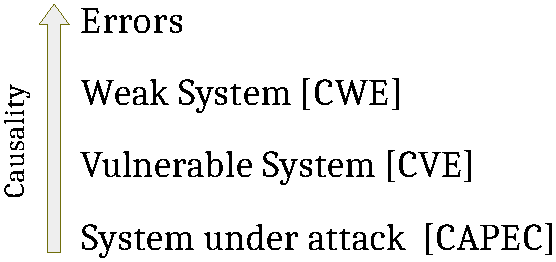
\includegraphics[width=.7\columnwidth]{causality.pdf}
	\caption{Etiology of cybersecurity}
	\label{fig:causality}
\end{figure}

Our literature review shows that most of the definitions relates insecurity to
dis-honesty (also called maliciousness or adversarial) of an agent (often
called adversary or attacker). This, however, just moves the problem of
defining what cybersecurity is as the problem of defining what an dishonest
agent can or cannot do in a system\footnote{where an agent is any virtual or
physical entity of the system or using the system (e.g. a device, a software,
or a human being) and dishonesty is not necessarily related to malicious
motivation but also to incompetence or lack of skills.} As in the Dolev-Yao
theory, we may correlate ``being dishonest'' to ``not following the intended
behavior/rules''.  In the case of a generic system, a dishonest agent is,
therefore, any agent that doesn't follow the intended behavior (or
functionality or logic) of the system.  Given the generality of the definition,
and its high level of abstraction, we may conclude that the hypothesis seems
evident. For example, a software can be considered an agent of the system and
whenever it has a bug, it can be exploited causing an Incident. However, this
hypothesis has lead to the un-testable conclusion that the dishonest behaviors
of agents cannot be defined in general (e.g. due to the heterogeneity of agents
and systems) and that huge repository of dishonest behaviors should be kept as
definition, such as CAPEC\cite{MITRE2020CAPEC}; or that dishonesty of an agent
with respect to a security protocol should be defined as a number of predefined
actions as in
\cite{Turuani2006clatse,Basin2005ofmc,Armando2016satmc,Rocchetto2017interpolation}
(to name a few). As depicted in Figure~\ref{fig:causality}, in order to define
a theory on cybersecurity and on the malicious behaviors of agents we noticed
that Attack Patterns (or Attacks) are caused-by the presence of Vulnerabilities
in the system. Those Vulnerabilities are, in turn, cause-by the presence of
Weaknesses in the system.  Weaknesses are Errors in the design or
implementation of a system.  Therefore, a theory on cybersecurity should first
predict the Errors in a system design.

\section{Security Hypothesis -- ABF Theory of Agents}\label{sec:hypothesis}
In order to address the problem raised by Herley, we shall define how to
distinguish between a secure and an insecure system. While most of the
literature have correlated the problem of in-security
to the maliciousness of agents interacting with the system, we show that
security doesn't seem to stem from a malicious nature but, rather, insecurity
raises from the lack of well-defined security requirements for the development
process of a system. We argue that the high number of security vulnerability
reported today are simply the realization of potential system configurations,
which deviate from the nominal behavior because the \emph{intended (or
nominal) behavior} of the system is not precisely defined in the specification
at the very early stages of the engineering process.

As a reference, we consider the following steps of the engineering process
and our objective is to be able to predict the security requirements
instead of axiomatically assume them.
\begin{enumerate}
	\item \emph{System Specification}, where the \emph{functional and physical requirements} are defined
	\item \emph{Architecture Design}, where the specification is structured into \emph{functional and physical architectures}
	\item \emph{Security Risk Assessment}, where the potential \emph{weaknesses} (errors)
		are identified and, consequently, \emph{security requirements} are
		captured.
	%\item \emph{Design Refinement}, where the physical and functional
	%	architectures are extended with \emph{mitigations} for the
	%	weaknesses. Mitigations at this step details the semantics of
	%	the functional blocks (behaviors), the data flow, and communication logic.
	%\item \emph{Verification of Security Requirements}, where the data flow, behaviors, and communication protocols are verified against the security requirements.
\end{enumerate}
Given that, in our investigation, we changed the focus from the attacker to the
potential designs of a system, we start by defining a general framework for the definition
of a system. On top of this framework we will identify system weaknesses as potential
design errors.

\subsection{Systems and Multi-Agent Systems}\label{sec:system}
The ISO/IEC/IEEE 15288:2015 (System Life Cycle Processes) provides a definition
of system as ``A combination of interacting elements organized to achieve one
or more stated purposes.''\autocite{ISO201515288}.  Therefore, a system can be
considered as a single agent where its interacting elements are the
constituents of the agent itself. For the sake of simplicity we first define a
system as an agent and then extend the definition to a ``combination of
interacting'' agents.  

There is no agreement between the research communities (e.g.
Multi-Agent-System, Epistemic Logic) on which are the constituent of an agent
as a system. However, the same ideas revolved around for thousands of years.
Some relevant examples for our objective are the following\footnote{
It is interesting to notice that 
in \autocite{Empiricus1990Pyrrhonism}, the author states: ``The
 logical criterion also may be used in three senses -- of the
 agent, or the instrument, or the ``according to what''; the
 agent, for instance, may be a man, the instrument either sense
 perception or intelligence, and the ``according to what'' the
 application of the impression ``according to'' which the man
 proceeds to judge by means of one of the aforesaid
 instruments.''. The author than proceeds showing that
 even in this framework, knowledge still is non-apprehensible.
}.
\begin{itemize}
	\item In \autocite{Hintikka1962knowledge}, Hintikka describes the
		difference between Knowledge and Belief (as epistemological
		concepts), and the whole Doxastic logic defines in details how
		Beliefs can be formalized.
	\item In \autocite{Hintikka1993Information}, Hintikka describes the concept
		of Information and the difference with Knowledge and Belief.
	\item In \autocite{Santaca2016abf}, the authors defines an agent as a
		tuple of Assertions, Beliefs, and Facts.
\end{itemize}
For our argument, as in \autocite{Santaca2016abf}, an agent is composed by its
knowledge, beliefs, and the information or assertions it provides; where
knowledge is defined, as in \autocite{Steup2020epistemology}, as a set of
proposition known by an agent, such that: (i) knowledge requires belief, (ii)
knowledge require truth, (iii) knowledge must be \emph{properly justified}, and
the only objective of Information is to exchange beliefs between agents.  As
defined in \autocite{Hintikka1993Information}, ``Information is specified by
specifying which alternatives concerning the reality it admits and which
alternatives excludes''. This means that if we consider a propositional
variable (which admits the two alternatives True/False) its information is
defined as Believed to be True/False and not Believed to be the opposite.  Due
to the definition of Information and then with its relation to the
probabilistic correlation to truth/reality, we consider information in relation
with an agent's beliefs. Similarly, we consider beliefs to define the actual
behavior of an agent or a system.

The difference between Knowledge and Information as used by Hintikka and Facts
and Assertions as used in \autocite{Santaca2016abf} are not precisely discussed
in \autocite{Santaca2016abf}.  Furthermore, those epistemological concepts are
difficult to define
\autocite{Gettier2012knowledge}\footnote{``\emph{Theaetetus}: [\ldots] He said
that knowledge was true opinion accompanied by reason, but that unreasoning
true opinion was outside of the sphere of knowledge; and matters of which there
is not a rational explanation are unknowable -- yes, that is what he called
them -- and those of which there is are knowable. [\ldots] \emph{Socrates}:
[\ldots] the primary elements of which we and all else are composed admit of no
rational explanation; for each alone by itself can only be named, and no
qualification can be added, neither that it is nor that it is not, for that
would at once be adding to it existence or non-existence, whereas we must add
nothing to it, if we are to speak of that itself alone.  [\ldots]'' Plato --
Theaetetus 201 \autocite{Plato1914Plato}}.  For example, Hintikka in
\autocite{Hintikka1993Information} states that ``A purely logical definition of
information is impossible''. A detailed formalization of those concepts is out
of the scope of this paper. We now define them abstractly, inspired by the
ABF-theory  defined in \autocite{Santaca2016abf} and, in
Section~\ref{sec:theory} we detail them as engineering concepts.
\begin{enumerate}
	\item We consider Information only when the intention of exchanging 
		that Information is from a sender to 
		recipient is defined; and we call it \emph{Assertion}  
	\item Similarly, the portion of Beliefs we consider for system
		engineering is the one that builds (input) or describes
		(output) the behavior of an agent (strategy rules
		\footnote{``The logical structure of information is one of the
		most basic and one of the most basic and one of the simplest
		thing in the wide and wonderful world of logical analysis. This
		point can be put in a deeper perspective. A distinction
		[\ldots] ought to be made [--] between two kinds of rules (or
		principles) in any strategic activity like knowledge seeking.
		On the one hand you have the rules that define the game, e.g.
		how chessmen are moved on a board. The can be called
		\emph{definitory} rules.  They must be distinguished from rules
		[\ldots] that deal with what is better and what is worse in the
		game in question.  Definitory rules do not say anything about
		this subject. Rules which do can be called \emph{strategic
		rules}'' -- Hintikka in \autocite{Hintikka1993Information}}),
		and
	\item We consider a set of axiomatic \emph{Facts} (definitory
		rules\fixnote{mr}{facts are definitory rule, as they don't
		define how a real system is finally implemented (currently) but
		how it should, trough a series of requirements which may not be
		respected, through insecurity, in the implemented system})
		instead of considering the more general epistemic definition of
		Knowledge. Specifically, Facts describes:
		\begin{itemize}
			\item The functional architecture of each agent
			\item The physical/structural (HW/SW) architecture of each
				subsystem of agents and agent within a
				subsystem
		\end{itemize}
\end{enumerate}
We give a graphical representation of (sub-)system and agent in Figure~\ref{fig:system-agent}
\fixnote{mr}{remove ``functional behavior'' in the figure and leave only ``behavior''}.

\begin{figure}[t]
	\centering
	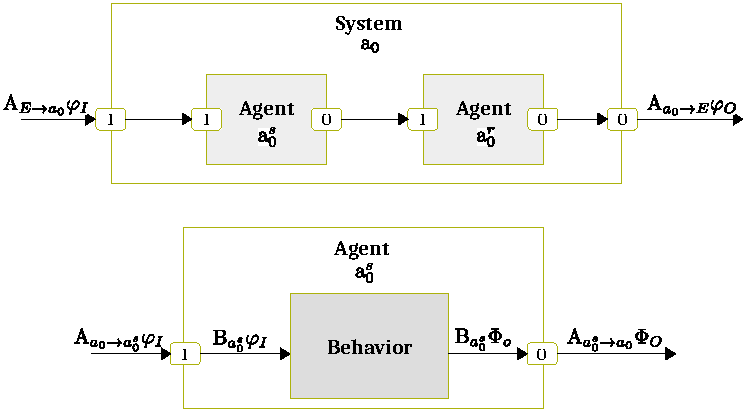
\includegraphics[width=.9\columnwidth]{system-agent.pdf}
	\caption{Example of system and agent structure}
	\label{fig:system-agent}
\end{figure}

\subsection{Mereo-topological Reasoning}
\begin{table*}[t]
\centering
\begin{tabular}{ccclll} 
\rota{\textbf{RCC3}}&\rota{\textbf{RCC5}}&\rota{\textbf{RCC8}}&\textbf{Terminology} & \textbf{Notation} & \textbf{Definition} \\
\hline
&&&Connects with 			& $\mathit{C}(\mathit{X},\mathit{Y})$ 		& $\mathit{X}\subseteq \mathit{Y}$ \\
&&&Disconnected from		& $\neg \mathit{C}(\mathit{X},\mathit{Y})$		& $\mathit{X}\not\subseteq \mathit{Y}$\\
&&&Part of				& $\mathit{P}(\mathit{X},\mathit{Y})$		& $\forall \mathit{Z} ~\mathit{C}(\mathit{Z},\mathit{X}) \rightarrow \mathit{C}(\mathit{Z},\mathit{Y})$\\
&&&Overlaps			& $\mathit{O}(\mathit{X},\mathit{Y})$		& $\exists \mathit{Z} ~\mathit{P}(\mathit{Z},\mathit{X})\wedge \mathit{P}(\mathit{Z},\mathit{Y})$\\
\Tdot&&&  \textbf{Overlaps Not Equal} 	& $\mathit{ONE}(\mathit{X},\mathit{Y})$		& $\mathit{O}(\mathit{X},\mathit{Y}) \land \neg \mathit{EQ}(\mathit{X},\mathit{Y})$ \\
\Tdot&\Tdot&\Tdot& \textbf{Equal to} 		& $\mathit{EQ}(\mathit{X},\mathit{Y})$  		& $\mathit{P}(\mathit{X},\mathit{Y}) \wedge \mathit{P}(\mathit{Y},\mathit{X})$\\
\Tdot&\Tdot&\Tdot& \textbf{DiscRete from} 		& $\mathit{DR}(\mathit{X},\mathit{Y})$		& $\neg \mathit{O}(\mathit{X},\mathit{Y})$\\
&\Tdot&\Tdot&\textbf{Partial-Overlap}	& $\mathit{PO}(\mathit{X},\mathit{Y})$ 		& $\mathit{O}(\mathit{X},\mathit{Y})\wedge \neg \mathit{P}(\mathit{X},\mathit{Y}) \wedge \neg \mathit{P}(\mathit{Y},\mathit{X})$\\ 
&\Tdot&&\textbf{Proper-Part-of} 	& $\mathit{PP}(\mathit{X},\mathit{Y})$ 		& $\mathit{P}(\mathit{X},\mathit{Y})\wedge \neg \mathit{P}(\mathit{Y},\mathit{X})$\\ 
	&\Tdot&&\textbf{Proper-Part-of-\textit{\textbf{i}}nverse} & $\mathit{PPi}(\mathit{X},\mathit{Y})$ 		& $\mathit{P}(\mathit{Y},\mathit{X}) \wedge \neg \mathit{P}(\mathit{X},\mathit{Y})$\\
&&\Tdot&\textbf{Externally Connected} 	& $\mathit{EC}(\mathit{X},\mathit{Y})$ 		& $\mathit{C}(\mathit{X},\mathit{Y}) \wedge \neg\mathit{O}(\mathit{X},\mathit{Y})$\\ 
&&\Tdot&\textbf{Tangential PP} 	& $\mathit{TPP}(\mathit{X},\mathit{Y})$ 		& $\mathit{PP}(\mathit{X},\mathit{Y})\wedge\exists\mathit{Z}~[\mathit{EC}(\mathit{Z},\mathit{X}),\mathit{EC}(\mathit{Z},\mathit{Y})]$\\ 
&&\Tdot&\textbf{Tangential PPi} 	& $\mathit{TPPi}(\mathit{X},\mathit{Y})$ 		& $\mathit{TPP}(\mathit{Y},\mathit{X})$\\ 
&&\Tdot&\textbf{Non-Tangential PP} 	& $\mathit{NTPP}(\mathit{X},\mathit{Y})$ 		& $\mathit{PP}(\mathit{X},\mathit{Y})\wedge\neg\exists\mathit{Z}~[\mathit{EC}(\mathit{Z},\mathit{X}),\mathit{EC}(\mathit{Z},\mathit{Y})]$\\ 
&&\Tdot&\textbf{Non-Tangential PPi} 	& $\mathit{NTPPi}(\mathit{X},\mathit{Y})$ 		& $\mathit{NTPP}(\mathit{Y},\mathit{X})$\\ 
\end{tabular}
\caption{RCC3, RCC5, and RCC8 relations between Regions $X$, $Y$ and $Z$ ~\label{tab:rcc358}~\label{tab:rcc}}
\end{table*}

Similarly to\autocite{Santaca2016abf}, we define agents as a meronomy (an
hierarchy of Part-Whole relations) over the constituent that we previously defined
(assertions, beliefs, and facts), based on a standard definition of mereology,
i.e. based on the definition of Parthood relation between \emph{Parts}.  Due to
the necessity of considering different types of Part (as we'll show afterwards)
we extend the mereology to a
mereo-topology\autocite{Smith1996mereotopology,Varzi1994mereotopology,Rachavelpula2017mereotopology},
considering the relations in Table~\ref{tab:rcc358}.  For the sake of
readability, we use the term \emph{Region} both to refer to a mereological Part
and to a topological Region.  Our aim is to create a meronomy
instead of the taxonomies such as the one provided
in\autocite{NIST2020NVD,MITRE2020CVE} with the
CVSS\autocite{Mell2007CVSS} scoring system.  

A mereotopology, as defined e.g. in\autocite{Rachavelpula2017mereotopology}, is
an ordered mathematical structure where the basic relation between Regions is
the reflexive and symmetric\fixnote{mr}{I guess it must be monotonic as defined
in\autocite{Rachavelpula2017mereotopology} but I don't find it consistently in
other papers.} \emph{Parthood} relation $\subseteq$.  
\begin{definition}{\bf Parthood --}\label{def:parthood}
Given any pair of mereotopological Regions $X$ and $Y$,
	\begin{enumerate}[noitemsep]
		\item Reflexivity: $\forall X.~ (X\subseteq X)$
		\item Symmetry: $\forall X, Y.~ (X\subseteq Y \Rightarrow Y\subseteq X)$
	\end{enumerate}
\end{definition}

The Parthood relation orders a universe of agents $\agentuniverse$ by defining the so called
\emph{Connects with} (see in Table~\ref{tab:rcc358}) relation between Regions.
We use the
Region Connection Calculus (RCC), as defined
in~\cite{bennettLogics,improvingRCC}, to provide an axiomatization of the
mereo-topological concepts. In its broader definition, the RCC theory is composed
by eight axioms, and is known as RCC8. In the text, for brevity, 
we will often focus only on RCC5 (without
loss of generality) by not considering tangential connections between spatial
Regions. In Table~\ref{tab:rcc}, we
summarize the axioms of the Region Connection Calculus (see, e.g., \autocite{Grutter2008rcc}).
We can now define a system over the mereotopology using the RCC calculus, as follows.

\begin{definition}{\bf System State --}\label{def:opsystem}
	A CPS system (or a sub-system) state is defined as the tuple
	$s=\langle\rcc(\factRegion,\beliefRegion),\rcc(\factRegion,\assertionRegion),\rcc(\beliefRegion,\assertionRegion)\rangle$,
	where $\assertionRegion,\beliefRegion,\factRegion$, are regions of
	assertions, beliefs (i.e. the beliefs generated by the behavior), and
	facts expressed as requirements respectively.
\end{definition}

As already presented in \autocite{Santaca2016abf} it follows that, defining
a system (or an operational system) with a fixed number of regions, there exist
an upper-bound to the number of possible configuration of a system, defined by
the possible relations between the different regions.
For completeness, we report in the next paragraph 
the calculation done in \autocite{Santaca2016abf}.

\paragraph{Number of different configurations of a system}
The general formula to calculate the number of different types of agents is
$r^{\binom{n}{k}}$, where $r$ is the number of relations with arity $k$,
between $n$ different sets, where $r^e$ is the number of permutation of $r$
relations over $e$ elements with repetitions, with $e$ being the number of
$k$-ary combinations of $n$ sets, $\binom{n}{k}$.
In our case, $\binom{n}{k}=3$ since we consider $3$ sets
($\assertionRegion,\beliefRegion,\factRegion$), and all the relations
considered in the RCC are binary.  Hence, using RCC5 (with five different
spatial relations) over three sets, we can theoretically define up to 125
different type of agents. However, only 54 of the 125 (as showed in
\cite{improvingRCC}) combinations are topologically correct with respect to
the definition of the relations of RCC5. Generalizing to all the RCCs:

\begin{itemize}%[nosep]
\item \emph{RCC3} --- theoretical: $3^3=27$,  correct: 15 
\item \emph{RCC5} --- theoretical: $5^3=125$, correct: 54
\item \emph{RCC8} --- theoretical: $8^3=512$, correct: 193
\end{itemize}

Hence, even if considering a different number of sets than the three
$\assertionRegion$, $\beliefRegion$ and $\factRegion$ exponentially affects
the number of theoretical agents, the application of RCC downscales that number
of a factor that ranges from 1.8 to 2.5. In addition, using RCC5 we consider
3.6 times more (different) types of agents than RCC3, but using RCC8 would
allow us to consider 3.5 times more different agents.
In the quantitative evaluation of a single agent, depicted in Figure~\ref{fig:quantitative},
we argue that only 1 configuration represents the nominal (expected) behavior 
of the agent while the other configurations are either impossible to 
implement or diverge from the intended nominal behavior. We note 
that, the numbers reported here do not consider the details of the
engineering process and should be considered a limit of an abstract 
representation of the system.
\begin{figure}[t]
	\centering
	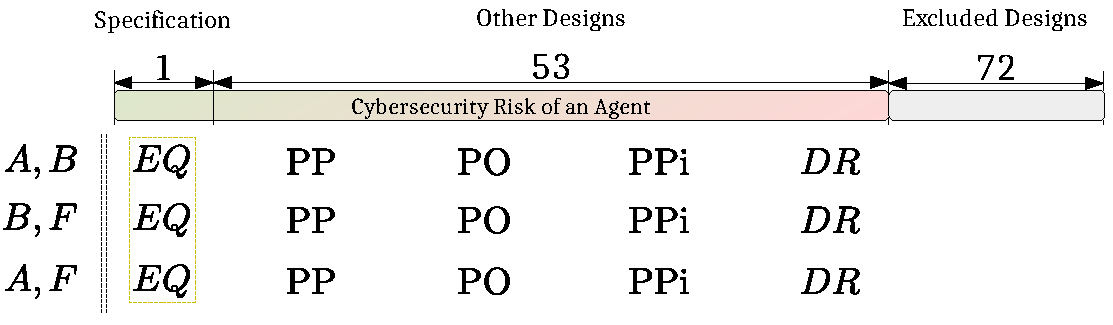
\includegraphics[width=\columnwidth]{quantitative.pdf}
	\caption{Cybersecurity risk for a single agent}
	\label{fig:quantitative}
\end{figure}

\subsection{Qualitative Evaluation of Agent Space in $\abf$}\label{sec:agentspace}
While a quantitative analysis reveals how many possible configurations of an
agent (i.e. a system) exist w.r.t. the $\abf$ theory (i.e. $54/125$ in RCC5), a
qualitative analysis of the different configurations describes the
configurations allowed by the $\abf$ theory, and how those configurations can
be categorized.  In Table~\ref{tab:5com}, we provide the generic composition
table of RCC5 over 3 regions instantiated over $\abf$, which shows the whole
state space for a single agent. The color coding of the table represents the
security risk related to a generic agent. 

As depicted in Figure~\ref{fig:soundness}, the relation between Facts, and
Assertions and Behavior defines the soundness of the design (admissible
configurations of Assertions, Behaviors and, in turn, Beliefs) w.r.t. the
specification (what the specification mandates, such as by the nature of the
physical/functional architectural models). We categorize agents by first
analyzing the relations between each pair of Regions defining an agent (i.e.
$\abf$), and then we categorize the different agents as tuple of the three
Regions.  For the sake of simplicity, soundness is opposed to non-soundness in
the following, however, with the RCC one should consider different ``degrees''
of non-soundness. For example, in RCC5, if we consider EQ between two Regions
as representing soundness, DR over the same Regions represents non-soundness;
while PP, PO, PPi represents the different degrees of non-soundness.  A similar
argument can be done for completeness.  \fix{mr}{it's missing the relation with
equivalence. missing parallelism with knowledge-belief/assertion (see slide
v-research-demo)}
\begin{figure}[t]
	\centering
	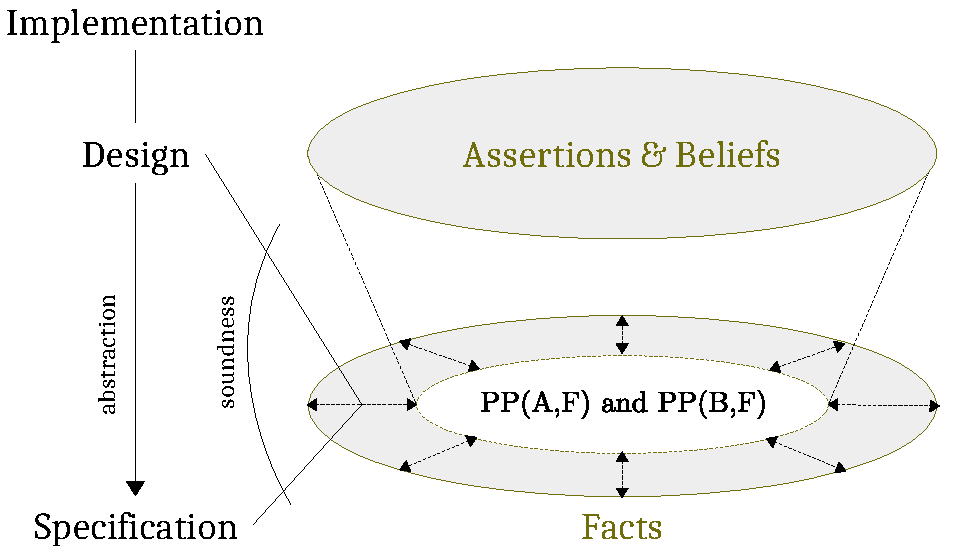
\includegraphics[width=\columnwidth]{soundness.pdf}
	\caption{Example relation between Facts, and Assertions and Beliefs}
	\label{fig:soundness}
\end{figure}

\paragraph{\Rcc{$\assertionRegion$}{$\beliefRegion$} -- Collaboration} In order
to reason on the relation between assertions and behavior we first need to
consider that, by definition, assertions are defined as transfer of information
between two agents, e.g., $a$ and $b$.  Therefore, as depicted in
Figure~\ref{fig:system-agent}, an agent has two main categories of assertions,
input and output assertions.  Given an agent $a$ and a collection of asserted
predicates $\Phi$, the Input assertions are those received by $a$ from an agent
$s$ acting as a sender, $\rassert{s}{a}{\Phi}$; similarly, output assertions
are sent from $a$ to a receiver $r$, $\rassert{a}{r}{\Phi}$. We shall consider
two pairs of regions\footnote{``I am not asserting, as Lotze did, that a
relation between $X$ and $Y$ consists of a quality in $X$ and a quality in $Y$
-- a view which I regard as quite indefensible. -- I assert that a relation $Z$
between $X$ and $Y$ involves the existence in $X$ of the quality ``having the
relation $Z$ to $Y$'' so that a difference of relations always involves a
difference in quality, and a change of relations always involves a change of
quality.'' --  Ellis J. McTaggart, The Unreality of
Time\autocite{Mctaggart1908unreality}}: 
\begin{itemize}
	\item \Rcc{$\assertionRegion_{s\rightarrow a}$}{$\beliefRegion$},
		where the relation between Input-assertions and behavior
		describes the soundness of the execution of the functional
		architecture w.r.t. input elicitation. With more details, the
		ideal specification of the functional architecture, along with
		the expected inputs, defines the functional behavior of an
		ideal system.  If all the inputs (Assertions) are correctly
		handled in the functional specification (behavior) the
		specification is complete. 

	\item \Rcc{$\assertionRegion_{a\rightarrow r}$}{$\beliefRegion$},
		where the relation between behavior and outputs describes the
		completeness of the behavior defined in the specification
		w.r.t. the input elicitation.  With more details, if all the
		outputs (assertions) of the functional architecture can be
		produced, the functional architecture is complete.
\end{itemize}


\paragraph{\Rcc{$\assertionRegion$}{$\factRegion$} and
\Rcc{$\beliefRegion$}{$\factRegion$} -- Honesty and Competence} While
Assertions and Beliefs generated by the Behavior determines how a system should
work, and the relation between the two defines the quality (i.e. the
completeness w.r.t the specification) of the agent, the relation of Assertions
and Behavior with Facts determines the quality with respect to the nominal
(specified) system.  Given that Facts defines what must be true in the system,
the relation of Assertions an Facts determines the degree of quality between
the information circulating in a system (or within an agent) and
reality\fixnote{mr}{assertions are reality while facts are dogmatic assertions
at specification level, i.e. requirements}.  Since the transfer of information
through Assertions generates Beliefs, a dishonest agent may circulate false
information, generating false Beliefs.  We note that it is often implied that
the intention behind circulating false information discerns a dishonest and an
incompetent agent, however, we consider honesty related to sharing
truths\footnote{``[\ldots] truth exists only in the good man, but the true in
the bad man as well; for it is possible for the bad man to utter something
true.'' Sextus Empiricus, Outlines of Pyrrhonism,
II-83\autocite{Empiricus1990Pyrrhonism}}.  The relation between Beliefs and
Facts determines the competence (on the subjects defined by the Facts) of an
agent (i.e. the more competent an agent is, the more likely a Belief of that
agent is true).

\subsubsection{$\abf$ Security Enumeration (SE)} The following security
requirement for a CPS specification can be summarized:
\begin{enumerate}
	\item[SE-$1$] Proper interaction between correctly-behaving agents (in
		contrast with the ``Improper Interaction Between Multiple
		Correctly-Behaving Entities'' defined by the CWE--$435$ as one
		of the top ``view'' of the ``research concepts'' in
		\autocite{MITRE2020CWEresearch}) is defined as
		$\eq{\assertionRegion_a}{\beliefRegion_a}$ for an agent $a$
		while can be detailed as follows when multiple agents are
		considered.
	\begin{enumerate}
		\item[SE-$1.1$] The equality relation
			$\eq{\assertionRegion_{s\rightarrow
			a}}{\beliefRegion_a}$ describes the intended secure
			behavior as: the beliefs generated by the behavior of
			the functional architecture shall be complete w.r.t.
			the specified inputs of the agent. Therefore, \emph{the
			assertions received by an agent or a system shall be
			compliant with the expected inputs of the functional
			architecture}. For example, the inputs of the user of a
			SW must be sanitized to exclude deviations w.r.t. the
			expected inputs of the functions implemented in the SW.
			Another example is the type checking between allowed
			inputs and expected inputs.
		\item[SE-$1.2$] Similarly, the equality relation
			$\eq{\assertionRegion_{a\rightarrow
			r}}{\beliefRegion_a}$ defines that the outputs of an
			agent $a$ shall be the outputs of the functional
			architecture.
	\end{enumerate}
	\item[SE-$2$]Sufficient Control Flow Management (in contrast with
		the ``Insufficient Control Flow Management'' defined by MITRE
		in the CWE--$691$ as one of the top ``view'' of the ``research
		concepts'' in\autocite{MITRE2020CWEresearch}) is defined as
		$\eq{\assertionRegion}{\factRegion}$.
	\item[SE-$3$] Correct Calculation (in contrast with the ``Improper
		Calculation'' defined by MITRE in the CWE--$682$ as one of the
		top ``view'' of the ``research concepts''
		in\autocite{MITRE2020CWEresearch}) is defined as
		$\eq{\beliefRegion}{\factRegion}$.
\end{enumerate}

We are now in the position to define what a secure system is (with respect to
the $\abf$-theory) and, based on that definition, what the security risk is and
how to quantify it in a risk matrix.
\begin{definition}{\bf Security of a System or an Agent --}\label{def:security}
	A secure system is a system where SE-$1$, SE-$2$, and SE-$3$ holds for
	each agent composing the system.
\end{definition}
The ISO 31000 consider risk as the ``effect of uncertainty on objectives'' and
the refers both of positive and negative consequences of uncertainty.
Accordingly, we consider risk as follows. 
\begin{definition}{\bf Risk --}
The whole space of potential designs of a specification with respect to the
	$\abf$-theory.
\end{definition}
The definition of Risk leads to the risk matrix in
Figure~\ref{fig:quantitative}, defined as follows.
\begin{definition}{\bf Risk Matrix --}
	The risk matrix is a function between the three relations
	$s=\langle\rcc(\factRegion,\beliefRegion),\rcc(\factRegion,\assertionRegion),\rcc(\beliefRegion,\assertionRegion)\rangle$,
	where the maximum risk is defined by the $DR$ relation between the
	three groups of Regions, and the minimum risk by the $EQ$ relation over
	the same Regions. In between the two extremes, the granularity of
	possible intermediate configuration is defined by the calculus used
	(RCC5 in our case).
\end{definition}
We note that often the risk matrix is defined by the relation between
likelihood and impact which we discuss in the next section.

\begin{table*}[t]
\centering
\begin{adjustbox}{width=.6\textwidth}
\begin{tabular}{r||c|c|c|c|c} 
& \dr{$\assertionRegion$}{$\beliefRegion$} & 
	\po{$\assertionRegion$}{$\beliefRegion$}& 
	\pp{$\assertionRegion$}{$\beliefRegion$} &
	\ppi{$\assertionRegion$}{$\beliefRegion$} & 
	\eq{$\assertionRegion$}{$\beliefRegion$} \\
\hline
\hline %dr
 \multirow{3}{*}{\dr{$\beliefRegion$}{$\factRegion$}} & 
	\cellcolor{abfred} & %dr
	\cellcolor{abf-rg-1}\dr{$\assertionRegion$}{$\factRegion$} & %po
	\cellcolor{abf-rg-2}\multirow{3}{*}{\dr{$\assertionRegion$}{$\factRegion$}} & %pp
	\cellcolor{abf-rg-3} \dr{$\assertionRegion$}{$\factRegion$}& % ppi
	 \cellcolor{abf-rg-4} \\ % eq
& \cellcolor{abfred}\all{$\assertionRegion$}{$\factRegion$}& %dr
	\cellcolor{abf-rg-1}\po{$\assertionRegion$}{$\factRegion$} & %po
	\cellcolor{abf-rg-2}\dr{$\assertionRegion$}{$\factRegion$} & %pp
	\cellcolor{abf-rg-3}\po{$\assertionRegion$}{$\factRegion$} & %ppi
	\cellcolor{abf-rg-4}\dr{$\assertionRegion$}{$\factRegion$}\\ % e q
 & \cellcolor{abfred}& %dr
	\cellcolor{abf-rg-1}\pp{$\assertionRegion$}{$\factRegion$} & %po
	\cellcolor{abf-rg-2}  & %pp
	\cellcolor{abf-rg-3}\pp{$\assertionRegion$}{$\factRegion$} & %ppi
	\cellcolor{abf-rg-4} \\ %eq
\hline %po
 \multirow{3}{*}{\po{$\beliefRegion$}{$\factRegion$}} &
	\cellcolor{abf-rg-1}\dr{$\assertionRegion$}{$\factRegion$} & %dr
	\cellcolor{abf-rg-2} & %po
	\cellcolor{abf-rg-3}\dr{$\assertionRegion$}{$\factRegion$} & %pp
	\cellcolor{abf-rg-4}\po{$\assertionRegion$}{$\factRegion$} & %ppi
	\cellcolor{abf-rg-5} \\ %eq
 & \cellcolor{abf-rg-1}\po{$\assertionRegion$}{$\factRegion$} & %dr
	\cellcolor{abf-rg-2} \all{$\assertionRegion$}{$\factRegion$} & %po 
	\cellcolor{abf-rg-3}\po{$\assertionRegion$}{$\factRegion$} & %pp
	\cellcolor{abf-rg-4}\ppi{$\assertionRegion$}{$\factRegion$} & %ppi
	\cellcolor{abf-rg-5} \po{$\assertionRegion$}{$\factRegion$}\\%eq
 & \cellcolor{abf-rg-1}\pp{$\assertionRegion$}{$\factRegion$} & %dr
	\cellcolor{abf-rg-2} &  %po
	\cellcolor{abf-rg-3}\pp{$\assertionRegion$}{$\factRegion$} & %pp
	\cellcolor{abf-rg-4}& %ppi
	\cellcolor{abf-rg-5}\\ %eq
\hline %pp
 \multirow{4}{*}{\pp{$\beliefRegion$}{$\factRegion$}} &
	\cellcolor{abf-rg-2}\dr{$\assertionRegion$}{$\factRegion$} & 
	\cellcolor{abf-rg-3}&
	\cellcolor{abf-rg-4} & %pp
	\cellcolor{abf-rg-5}\po{$\assertionRegion$}{$\factRegion$} & %ppi
	\cellcolor{abf-rg-6}\\ %eq
 & \cellcolor{abf-rg-2}\po{$\assertionRegion$}{$\factRegion$} & 
	\cellcolor{abf-rg-3}\po{$\assertionRegion$}{$\factRegion$} & 
	\cellcolor{abf-rg-4}\pp{$\assertionRegion$}{$\factRegion$} & %pp
	\cellcolor{abf-rg-5}\eq{$\assertionRegion$}{$\factRegion$} & %ppi
	\cellcolor{abf-rg-6}\pp{$\assertionRegion$}{$\factRegion$} \\ %eq
 & \cellcolor{abf-rg-2}\pp{$\assertionRegion$}{$\factRegion$} & 
	\cellcolor{abf-rg-3}\pp{$\assertionRegion$}{$\factRegion$} & 
	\cellcolor{abf-rg-4} & %pp
	\cellcolor{abf-rg-5}\pp{$\assertionRegion$}{$\factRegion$} & %ppi
	\cellcolor{abf-rg-6} \\ %eq
 & \cellcolor{abf-rg-2}&
 	\cellcolor{abf-rg-3} & 
	\cellcolor{abf-rg-4}& %pp
	\cellcolor{abf-rg-5}\ppi{$\assertionRegion$}{$\factRegion$} & %ppi
	\cellcolor{abf-rg-6} \\ %eq
\hline %ppi
 \multirow{3}{*}{\ppi{$\beliefRegion$}{$\factRegion$}} &
 	\cellcolor{abf-rg-3}\multirow{3}{*}{} &
 	\cellcolor{abf-rg-4}\dr{$\assertionRegion$}{$\factRegion$} &
 	\cellcolor{abf-rg-5}& %pp
 	\cellcolor{abf-rg-6}& %ppi
 	\cellcolor{abf-rg-7} \\ %eq
& \cellcolor{abf-rg-3}\dr{$\assertionRegion$}{$\factRegion$} &
 	\cellcolor{abf-rg-4}\po{$\assertionRegion$}{$\factRegion$} & 
 	\cellcolor{abf-rg-5}\all{$\assertionRegion$}{$\factRegion$}& %pp
 	\cellcolor{abf-rg-6}\ppi{$\assertionRegion$}{$\factRegion$}& %ppi
 	\cellcolor{abf-rg-7}\ppi{$\assertionRegion$}{$\factRegion$}\\ %eq
& \cellcolor{abf-rg-3} & 
	\cellcolor{abf-rg-4}\ppi{$\assertionRegion$}{$\factRegion$} & 
	\cellcolor{abf-rg-5} & %pp
	\cellcolor{abf-rg-6}& %ppi
	\cellcolor{abf-rg-7}\\ %eq
\hline %eq
	\eq{$\beliefRegion$}{$\factRegion$} & 
	\cellcolor{abf-rg-4}\dr{$\assertionRegion$}{$\factRegion$} & 
	\cellcolor{abf-rg-5} \po{$\assertionRegion$}{$\factRegion$} & 
	\cellcolor{abf-rg-6}\pp{$\assertionRegion$}{$\factRegion$} & %pp
	\cellcolor{abf-rg-7} \ppi{$\assertionRegion$}{$\factRegion$} & %ppi 
	\cellcolor{abfgreen} \eq{$\assertionRegion$}{$\factRegion$}  %eq
\end{tabular}
\end{adjustbox}
\caption{RCC5 composition table over 3 regions. The results show that there
exist 54 possible relations and the coloring anticipates the ideal risk matrix
(green the secure state with low risk, red the high risk state, and a gradient
of medium risk states). 
\all{$\assertionRegion$}{$\factRegion$} = \{\dr{$\assertionRegion$}{$\factRegion$}, \po{$\assertionRegion$}{$\factRegion$}, \pp{$\assertionRegion$}{$\factRegion$}, \ppi{$\assertionRegion$}{$\factRegion$}, \eq{$\assertionRegion$}{$\factRegion$}\}
\label{tab:5com}}
\end{table*}

\section{Prediction of Security Weaknesses}\label{sec:theory}
\begin{figure*}[t]
	\centering
	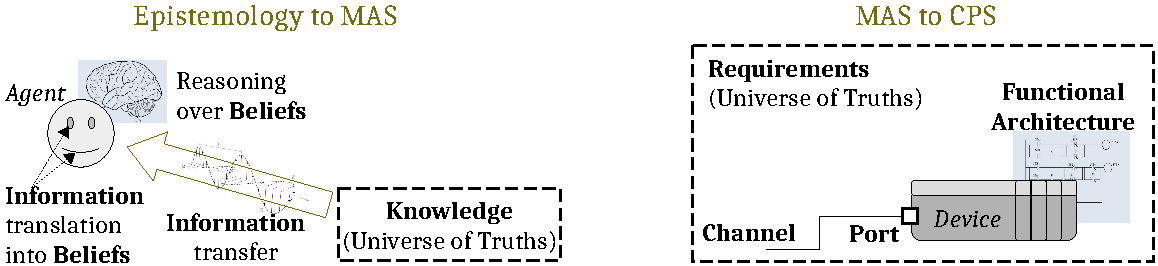
\includegraphics[width=.9\textwidth]{mashyp.pdf}
	\caption{asd}
	\label{fig:mashyp}
\end{figure*}

\paragraph{Fun, Behavior, Channels}

\section{Security Risk Assessment}\label{sec:secra}
\paragraph{Automated Security Requirements Extraction}

\section{Discussions}\label{sec:discussion}
\paragraph{Framework for Theory Falsification}
\paragraph{SPDL, Testing, and Falsification}
\paragraph{Relation with DY}
\paragraph{Abstraction Level}

\section{Conclusion and Future Works}
\begin{itemize}
	\item Verification
	\item Testing
\end{itemize}

\section*{Acknowledgment}
We thank Katia Santac\`a for the development of the initial ideas, and for
the helpful discussions that allowed us to make this step forward.

% trigger a \newpage just before the given reference
% number - used to balance the columns on the last page
% adjust value as needed - may need to be readjusted if
% the document is modified later
%\IEEEtriggeratref{8}
% The "triggered" command can be changed if desired:
%\IEEEtriggercmd{\enlargethispage{-5in}}

%\bibliographystyle{IEEEtran}
%\bibliography{../literature}
\printbibliography

\end{document}
